\documentclass[10pt]{beamer}
\usepackage{hyperref}
\usepackage{fontawesome}
\usepackage{graphicx}
\usepackage[english]{babel}

% ------------------------------------------------------------------------------
% Use the beautiful metropolis beamer template
% ------------------------------------------------------------------------------
\usepackage[T1]{fontenc}
\usepackage{fontawesome}
\usepackage{FiraSans} 
\mode<presentation>
{
  \usetheme[progressbar=foot,numbering=fraction,background=light]{metropolis} 
  \usecolortheme{default} % or try albatross, beaver, crane, ...
  \usefonttheme{default}  % or try serif, structurebold, ...
  \setbeamertemplate{navigation symbols}{}
  \setbeamertemplate{caption}[numbered]
  %\setbeamertemplate{frame footer}{My custom footer}
}

% ------------------------------------------------------------------------------
% minted
% ------------------------------------------------------------------------------
\usepackage{minted}

% ------------------------------------------------------------------------------
% tikz
% ------------------------------------------------------------------------------
\usepackage{tikz}
\usetikzlibrary{calc, arrows.meta, positioning, automata}

\usepackage{listings}


% ------------------------------------------------------------------------------
% The Document
% ------------------------------------------------------------------------------
\title{reachability analysis for continuous one counter automata}
\author{Lars Van Roy\\
\textit{dept. of Mathematics and Computer Science} \\
\textit{University of Antwerp}\\
lars.vanroy@student.uantwerpen.be}

\newcommand{\highlight}[1]{%
	\colorbox{blue!50}{$\displaystyle#1$}}

\usepackage{xcolor}
\definecolor{ForestGreen}{RGB}{34,139,34}

\begin{document}

\maketitle

\section{Problem overview}

\begin{frame}{Problem overview I}
	\begin{itemize}
	    \item Reachability analysis
	    \begin{itemize}
	    	\pause
	    	\item Are all conditional statements satisfiable
    	\end{itemize}
    	\pause
    	\item Explore set of values that a counter can have
    	\pause
    	\item Analysis of one-counter continuous automata
    	\pause
    	\item Only applicable to simple functions
	\end{itemize}
\end{frame}

\begin{frame}{Problem overview II}
	\begin{itemize}
		\item Only applicable to simple functions
		\begin{itemize}
			\pause
			\item Supported comparisons: $\leq, <, ==, \ne, >, \geq$
			\pause
			\item Supported operations: $+, -, =$
			\pause
			\item Restrictions only apply for counters
			\pause
			\item Counter must be of type integer
			\pause
			\item Conditions and operations on counters can be performed with
			\begin{itemize}
				\item Parameters
				\item Constants
			\end{itemize}
			\pause
			\item There can only be one consecutive counter
		\end{itemize}
	\end{itemize}
\end{frame}

\section{Approach}

\begin{frame}{Approach}
	\begin{figure}[h!]
		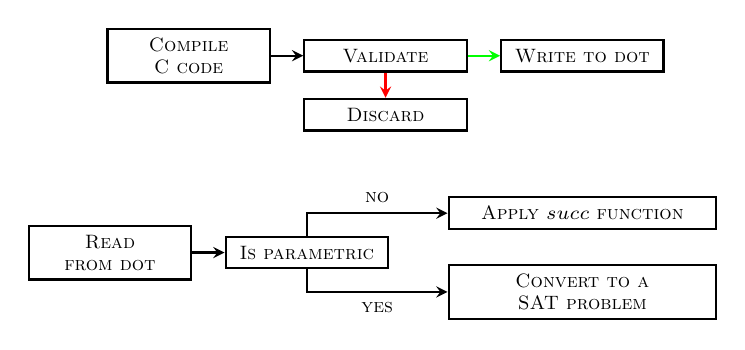
\begin{tikzpicture}[auto, >=latex, node distance = 1 cm]
			\tikzstyle{node} = [thick, draw=black, rectangle, font=\scriptsize\scshape, text width=5.2em, align=center]
			\tikzstyle{node2} = [thick, draw=black, rectangle, font=\scriptsize\scshape, text width=9em, align=center]
			\tikzstyle{arrow} = [thick,->,>=stealth]
			
			\node[node] 	at (1, 0)		(q1)	{Compile C code};
			\node[node] 	at (3.5, 0)		(q2)	{Validate};
			\node[node]		at (3.5, -0.75) (q3)	{Discard};
			\node[node]		at (6, 0)		(q4)	{Write to dot};
			
			\node[node]		at (0, -2.5)	(q5)	{Read from dot};
			\node[node]		at (2.5, -2.5)	(q6)	{Is parametric};
			\node[node2]	at (6, -2)		(q7)	{Apply $succ$ function};
			\node[node2]	at (6, -3)		(q8)	{Convert to a SAT problem};
			
			\draw [arrow] 			(q1) -> (q2);
			\draw [arrow, red] 		(q2) -> (q3);
			\draw [arrow, green] 	(q2) -> (q4);
			
			
			\draw [arrow] 			(q5) -> (q6);
			\draw [arrow] 			(q6) |- (q7) 	node	[near end, above]	{\scriptsize\scshape no};
			\draw [arrow] 			(q6) |- (q8)	node	[near end, below]	{\scriptsize\scshape yes};
		\end{tikzpicture}
	\end{figure}
\end{frame}

\begin{frame}{Reachability intervals}
	\begin{itemize}
		\only<1->{\item Interval representing possible counter values}
		\only<2->{\item Tracked for each of the nodes}
	\end{itemize}
	\vspace{1em}
	\only<3>{	
		\begin{figure}[h!]
			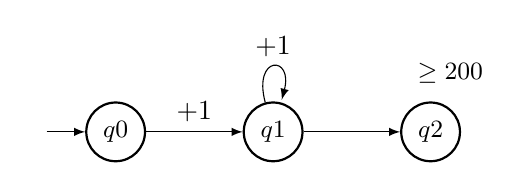
\begin{tikzpicture}[auto, >=latex, node distance = 1 cm]
				\tikzstyle{round} = [thick, draw=black, circle, font=\small]
				\tikzstyle{invis} = [draw=none, font=\small]
				
				\node[invis]			at (-1,0)		(q3)	{$ $};
				\node[round] 			at (0, 0) 		(q0) 	{$q0$};
				\node[round] 			at (2, 0) 		(q1) 	{$q1$};
				\node[round] 			at (4, 0) 		(q2) 	{$q2$};
				\node[invis] 			at (4.25, 0.75)	(q7) 	{$\geq 200$};
				
				\path[->]
				(q3)	edge				node {$ $}	(q0)
				(q0)	edge				node {$+1$}	(q1)
				(q1)	edge				node {$ $}	(q2)
				(q1)	edge [loop above]	node {$+1$}	(q1);
			\end{tikzpicture}
		\end{figure}
	}
	\only<4>{	
		\begin{figure}[h!]
			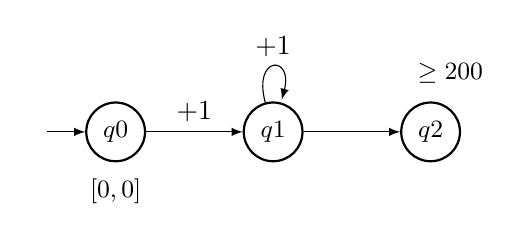
\begin{tikzpicture}[auto, >=latex, node distance = 1 cm]
				\tikzstyle{round} = [thick, draw=black, circle, font=\small]
				\tikzstyle{invis} = [draw=none, font=\small]
				
				\node[invis]			at (-1,0)		(q3)	{$ $};
				\node[round] 			at (0, 0) 		(q0) 	{$q0$};
				\node[round] 			at (2, 0) 		(q1) 	{$q1$};
				\node[round] 			at (4, 0) 		(q2) 	{$q2$};
				\node[invis] 			at (0, -0.75)	(q4) 	{$[0, 0]$};
				\node[invis] 			at (4.25, 0.75)	(q7) 	{$\geq 200$};
				
				\path[->]
				(q3)	edge				node {$ $}	(q0)
				(q0)	edge				node {$+1$}	(q1)
				(q1)	edge				node {$ $}	(q2)
				(q1)	edge [loop above]	node {$+1$}	(q1);
			\end{tikzpicture}
		\end{figure}
	}
	\only<5>{	
		\begin{figure}[h!]
			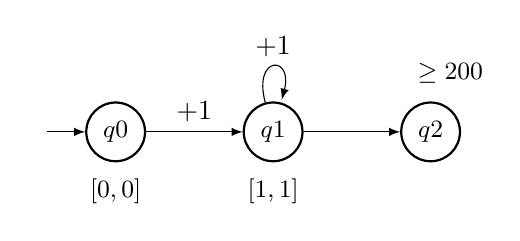
\begin{tikzpicture}[auto, >=latex, node distance = 1 cm]
				\tikzstyle{round} = [thick, draw=black, circle, font=\small]
				\tikzstyle{invis} = [draw=none, font=\small]
				
				\node[invis]			at (-1,0)		(q3)	{$ $};
				\node[round] 			at (0, 0) 		(q0) 	{$q0$};
				\node[round] 			at (2, 0) 		(q1) 	{$q1$};
				\node[round] 			at (4, 0) 		(q2) 	{$q2$};
				\node[invis] 			at (0, -0.75)	(q4) 	{$[0, 0]$};
				\node[invis] 			at (2, -0.75)	(q5) 	{$[1, 1]$};
				\node[invis] 			at (4.25, 0.75)	(q7) 	{$\geq 200$};
				
				\path[->]
				(q3)	edge				node {$ $}	(q0)
				(q0)	edge				node {$+1$}	(q1)
				(q1)	edge				node {$ $}	(q2)
				(q1)	edge [loop above]	node {$+1$}	(q1);
			\end{tikzpicture}
		\end{figure}
	}
	\only<6>{	
		\begin{figure}[h!]
			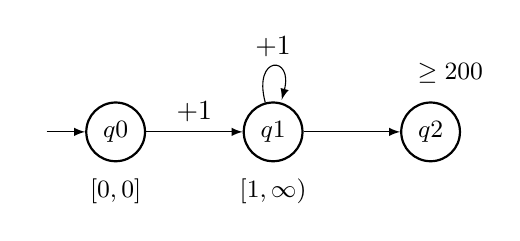
\begin{tikzpicture}[auto, >=latex, node distance = 1 cm]
				\tikzstyle{round} = [thick, draw=black, circle, font=\small]
				\tikzstyle{invis} = [draw=none, font=\small]
				
				\node[invis]			at (-1,0)		(q3)	{$ $};
				\node[round] 			at (0, 0) 		(q0) 	{$q0$};
				\node[round] 			at (2, 0) 		(q1) 	{$q1$};
				\node[round] 			at (4, 0) 		(q2) 	{$q2$};
				\node[invis] 			at (0, -0.75)	(q4) 	{$[0, 0]$};
				\node[invis] 			at (2, -0.75)	(q5) 	{$[1, \infty)$};
				\node[invis] 			at (4.25, 0.75)	(q7) 	{$\geq 200$};
				
				\path[->]
				(q3)	edge				node {$ $}	(q0)
				(q0)	edge				node {$+1$}	(q1)
				(q1)	edge				node {$ $}	(q2)
				(q1)	edge [loop above]	node {$+1$}	(q1);
			\end{tikzpicture}
		\end{figure}
	}
	\only<7>{	
		\begin{figure}[h!]
			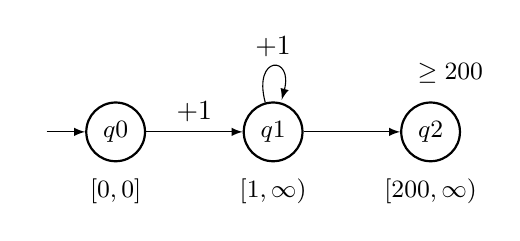
\begin{tikzpicture}[auto, >=latex, node distance = 1 cm]
				\tikzstyle{round} = [thick, draw=black, circle, font=\small]
				\tikzstyle{invis} = [draw=none, font=\small]
				
				\node[invis]			at (-1,0)		(q3)	{$ $};
				\node[round] 			at (0, 0) 		(q0) 	{$q0$};
				\node[round] 			at (2, 0) 		(q1) 	{$q1$};
				\node[round] 			at (4, 0) 		(q2) 	{$q2$};
				\node[invis] 			at (0, -0.75)	(q4) 	{$[0, 0]$};
				\node[invis] 			at (2, -0.75)	(q5) 	{$[1, \infty)$};
				\node[invis] 			at (4, -0.75)	(q6) 	{$[200, \infty)$};
				\node[invis] 			at (4.25, 0.75)	(q7) 	{$\geq 200$};
				
				\path[->]
				(q3)	edge				node {$ $}	(q0)
				(q0)	edge				node {$+1$}	(q1)
				(q1)	edge				node {$ $}	(q2)
				(q1)	edge [loop above]	node {$+1$}	(q1);
			\end{tikzpicture}
		\end{figure}
	}
\end{frame}

\section{Successor function}

\begin{frame}{Successor function I}
	\begin{itemize}
		\item Approach for non-parametric automata
		\pause
		\item Evaluate the reachability intervals iteratively
		\pause
		\item Acceleration to prevent infinite loops
	\end{itemize}
\end{frame}

\begin{frame}{Successor function II}
	\only<1>{
		\begin{gather*}
			\hspace{-6 pt} succ_i(p, q) := \bigcup \{(R_i(p, q) + (0, z]) \cap \tau(q)\,|\,(p,z,q) \in T, z>0\}\\
			\hspace{49 pt} \cup \bigcup \{(R_i(p, q) + [z, 0)) \cap \tau(q)\,|\,(p,z,q) \in T, z<0\}\\
			\hspace{51.8 pt} \cup \bigcup \{(R_i(p, q) + [0, 0]) \cap \tau(q)\,|\,(p,0,q) \in T, z=0\}
		\end{gather*}
		\begin{enumerate}
			\item {Generate the next interval for the edge going from p to q}
			\item Apply the edge operation to the current interval
			\item Ensure that the interval is within the node bounds
		\end{enumerate}
	}
	\only<2>{
		\begin{gather*}
			\hspace{-6 pt} \highlight{succ_i(p, q)} := \bigcup \{(R_i(p, q) + (0, z]) \cap \tau(q)\,|\,(p,z,q) \in T, z>0\}\\
			\hspace{49 pt} \cup \bigcup \{(R_i(p, q) + [z, 0)) \cap \tau(q)\,|\,(p,z,q) \in T, z<0\}\\
			\hspace{51.8 pt} \cup \bigcup \{(R_i(p, q) + [0, 0]) \cap \tau(q)\,|\,(p,0,q) \in T, z=0\}
		\end{gather*}
		\begin{enumerate}
			\item \textcolor{blue}{Generate the next interval for the edge going from p to q}
			\item Add the operation interval to the current reachability interval
			\begin{itemize}
				\item operation interval = (0, 1] * z
			\end{itemize}
			\item Ensure that the interval is within the node bounds
		\end{enumerate}
	}
	\only<3>{
		\begin{gather*}
			\hspace{-6 pt} succ_i(p, q) := \bigcup \highlight{\{(R_i(p, q) + (0, z])} \cap \tau(q)\,|\,(p,z,q) \in T, z>0\}\\
			\hspace{49 pt} \cup \bigcup \highlight{\{(R_i(p, q) + [z, 0))} \cap \tau(q)\,|\,(p,z,q) \in T, z<0\}\\
			\hspace{51.8 pt} \cup \bigcup \highlight{\{(R_i(p, q) + [0, 0])} \cap \tau(q)\,|\,(p,0,q) \in T, z=0\}
		\end{gather*}
		\begin{enumerate}
			\item Generate the next interval for the edge going from p to q
			\item \textcolor{blue}{Add the operation interval to the current reachability interval
				\begin{itemize}
					\item operation interval = (0, 1] * z
			\end{itemize}}
			\item Ensure that the interval is within the node bounds
		\end{enumerate}
	}
	\only<4>{
		\begin{gather*}
			\hspace{-6 pt} succ_i(p, q) := \bigcup \{(R_i(p, q) + (0, z]) \highlight{\cap \tau(q)}\,|\,(p,z,q) \in T, z>0\}\\
			\hspace{49 pt} \cup \bigcup \{(R_i(p, q) + [z, 0)) \highlight{\cap \tau(q)}\,|\,(p,z,q) \in T, z<0\}\\
			\hspace{51.8 pt} \cup \bigcup \{(R_i(p, q) + [0, 0]) \highlight{\cap \tau(q)}\,|\,(p,0,q) \in T, z=0\}
		\end{gather*}
		\begin{enumerate}
			\item {Generate the next interval for the edge going from p to q}
			\item Add the operation interval to the current reachability interval
			\begin{itemize}
				\item operation interval = (0, 1] * z
			\end{itemize}
			\item \textcolor{blue}{Ensure that the interval is within the node bounds}
		\end{enumerate}
	}
\end{frame}

\begin{frame}{Successor function III}
	\begin{itemize}
		\item Iteratively update intervals until no more changes occur
		\pause
		\item Only apply the $succ$ function to non-empty intervals
	\end{itemize}
\end{frame}

\begin{frame}[fragile]{Successor function IV}
\begin{minipage}[c]{0.49\textwidth}
\begin{lstlisting}[
		language=C, 
		basicstyle=\footnotesize, 
		numbers=left,
		stepnumber=1,]
int func() {
   for (int i;i < 11;) {
      if (i == 12) {
         return -1;
      }
      i += 2;
   }
   return 0;
}
\end{lstlisting}
\end{minipage}
\hfill
\begin{minipage}[c]{0.49\textwidth}
	\begin{figure}[h!]
		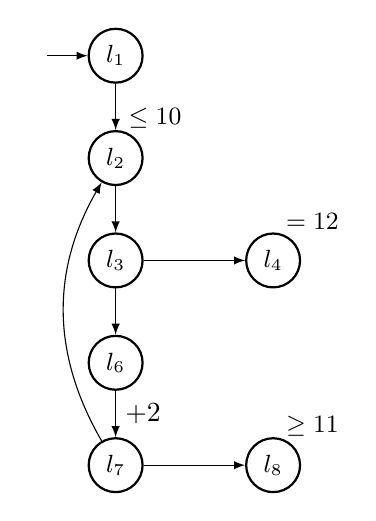
\begin{tikzpicture}[auto, >=latex, node distance = 1 cm]
			\tikzstyle{round} = [thick, draw=black, circle, font=\small]
			\tikzstyle{invis} = [draw=none, font=\small]
			
			\node[invis]			at (-1,0)		(q6)	{$ $};
			\node[round] 			at (0, 0) 		(q0) 	{$l_1$};
			\node[round] 			at (0, -1.3)	(q1) 	{$l_2$};
			\node[invis]			at (0.5, -0.8)	(c0)	{$\leq 10$};
			\node[round] 			at (0, -2.6)	(q2) 	{$l_3$};
			\node[round] 			at (2, -2.6) 	(q3) 	{$l_4$};
			\node[invis]			at (2.5, -2.1)	(c0)	{$= 12$};
			\node[round] 			at (0, -5.2)	(q4) 	{$l_7$};
			\node[round] 			at (0, -3.9)	(q7) 	{$l_6$};
			\node[round] 			at (2, -5.2)	(q5) 	{$l_8$};
			\node[invis]			at (2.5, -4.7)	(c1)	{$\geq 11$};
			
			\path[->]
			(q6)	edge				node {$ $}	(q0)
			(q0)	edge				node {$ $}	(q1)
			(q1)	edge				node {$ $}	(q2)
			(q2)	edge				node {$ $}	(q7)
			(q7)	edge				node {$+2$}	(q4)
			(q2)	edge				node {$ $}	(q3)
			(q4)	edge				node {$ $}	(q5)
			(q4)	edge [bend left]	node {$ $}  (q1);
		\end{tikzpicture}
	\end{figure}
\end{minipage}
\end{frame}


\begin{frame}[fragile]{Successor function V}
	\begin{minipage}[c]{0.60\textwidth}
		\only<1>{
			\begin{table}[h]
				\footnotesize
				\begin{tabular}{ |c|c|c| }
					\hline
					p		& q 	& $R_0$ 		\\
					\hline
					$l_1$	& $l_2$ & [0, 0] 		\\
					\hline
					$l_2$	& $l_3$ & $\emptyset$ 	\\
					\hline
					$l_3$	& $l_4$ & $\emptyset$ 	\\
					\hline
					$l_3$	& $l_6$ & $\emptyset$ 	\\
					\hline
					$l_6$	& $l_7$ & $\emptyset$ 	\\
					\hline
					$l_7$	& $l_2$ & $\emptyset$ 	\\
					\hline
					$l_7$	& $l_8$ & $\emptyset$ 	\\
					\hline
				\end{tabular}
				\centering
			\end{table}
		}
		\only<2>{
			\begin{table}[h]
				\footnotesize
				\begin{tabular}{ |c|c|c|c| }
					\hline
					p		& q 	& $R_0$ 		& $R_1$			\\
					\hline
					$l_1$	& $l_2$ & [0, 0] 		& [0, 0] 		\\
					\hline
					$l_2$	& $l_3$ & $\emptyset$ 	& [0, 0]		\\
					\hline
					$l_3$	& $l_4$ & $\emptyset$ 	& $\emptyset$ 	\\
					\hline
					$l_3$	& $l_6$ & $\emptyset$ 	& $\emptyset$ 	\\
					\hline
					$l_6$	& $l_7$ & $\emptyset$ 	& $\emptyset$ 	\\
					\hline
					$l_7$	& $l_2$ & $\emptyset$ 	& $\emptyset$ 	\\
					\hline
					$l_7$	& $l_8$ & $\emptyset$ 	& $\emptyset$ 	\\
					\hline
				\end{tabular}
				\centering
			\end{table}	
		}
		\only<3>{
			\begin{table}[h]
				\footnotesize
				\begin{tabular}{ |c|c|c|c|c| }
					\hline
					p		& q 	& $R_0$ 		& $R_1$			& $R_2$			\\
					\hline
					$l_1$	& $l_2$ & [0, 0] 		& [0, 0] 		& [0, 0] 		\\
					\hline
					$l_2$	& $l_3$ & $\emptyset$ 	& [0, 0]		& [0, 0] 		\\
					\hline
					$l_3$	& $l_4$ & $\emptyset$ 	& $\emptyset$ 	& $\emptyset$ 	\\
					\hline
					$l_3$	& $l_6$ & $\emptyset$ 	& $\emptyset$ 	& [0, 0]		\\
					\hline
					$l_6$	& $l_7$ & $\emptyset$ 	& $\emptyset$ 	& $\emptyset$	\\
					\hline
					$l_7$	& $l_2$ & $\emptyset$ 	& $\emptyset$ 	& $\emptyset$	\\
					\hline
					$l_7$	& $l_8$ & $\emptyset$ 	& $\emptyset$ 	& $\emptyset$	\\
					\hline
				\end{tabular}
				\centering
			\end{table}
			}
		\only<4>{
		\begin{table}[h]
			\footnotesize
			\begin{tabular}{ |c|c|c|c|c|c| }
				\hline
				p		& q 	& $R_0$ 		& $R_1$			& $R_2$			& $R_3$			\\
				\hline
				$l_1$	& $l_2$ & [0, 0] 		& [0, 0] 		& [0, 0] 		& [0, 0]		\\
				\hline
				$l_2$	& $l_3$ & $\emptyset$ 	& [0, 0]		& [0, 0] 		& [0, 0]		\\
				\hline
				$l_3$	& $l_4$ & $\emptyset$ 	& $\emptyset$ 	& $\emptyset$	& $\emptyset$	\\
				\hline
				$l_3$	& $l_6$ & $\emptyset$ 	& $\emptyset$ 	& [0, 0]		& [0, 0]		\\
				\hline
				$l_6$	& $l_7$ & $\emptyset$ 	& $\emptyset$ 	& $\emptyset$	& (0, 2]		\\
				\hline
				$l_7$	& $l_2$ & $\emptyset$ 	& $\emptyset$ 	& $\emptyset$	& $\emptyset$   \\
				\hline
				$l_7$	& $l_8$ & $\emptyset$ 	& $\emptyset$ 	& $\emptyset$	& $\emptyset$	\\
				\hline
			\end{tabular}
			\centering
		\end{table}
		}
		\only<5>{
		\begin{table}[h]
			\footnotesize
			\begin{tabular}{ |c|c|c|c|c|c|c| }
				\hline
				p		& q 	& $R_0$ 		& $R_1$			& $R_2$			& $R_3$			& $R_4$\\
				\hline
				$l_1$	& $l_2$ & [0, 0] 		& [0, 0] 		& [0, 0] 		& [0, 0]		& [0, 0]\\
				\hline
				$l_2$	& $l_3$ & $\emptyset$ 	& [0, 0]		& [0, 0] 		& [0, 0]		& [0, 0]\\
				\hline
				$l_3$	& $l_4$ & $\emptyset$ 	& $\emptyset$ 	& $\emptyset$	& $\emptyset$	& $\emptyset$\\
				\hline
				$l_3$	& $l_6$ & $\emptyset$ 	& $\emptyset$ 	& [0, 0]		& [0, 0]		& [0, 0]\\
				\hline
				$l_6$	& $l_7$ & $\emptyset$ 	& $\emptyset$ 	& $\emptyset$	& (0, 2]		& (0, 2]\\
				\hline
				$l_7$	& $l_2$ & $\emptyset$ 	& $\emptyset$ 	& $\emptyset$	& $\emptyset$   & (0, 2]\\
				\hline
				$l_7$	& $l_8$ & $\emptyset$ 	& $\emptyset$ 	& $\emptyset$	& $\emptyset$	& $\emptyset$\\
				\hline
			\end{tabular}
			\centering
		\end{table}
		}
	\end{minipage}
	\hfill
	\begin{minipage}[c]{0.39\textwidth}
		\begin{figure}[h!]
			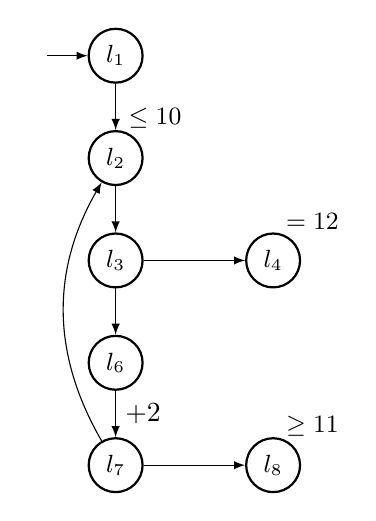
\begin{tikzpicture}[auto, >=latex, node distance = 1 cm]
				\tikzstyle{round} = [thick, draw=black, circle, font=\small]
				\tikzstyle{invis} = [draw=none, font=\small]
				
				\node[invis]			at (-1,0)		(q6)	{$ $};
				\node[round] 			at (0, 0) 		(q0) 	{$l_1$};
				\node[round] 			at (0, -1.3)	(q1) 	{$l_2$};
				\node[invis]			at (0.5, -0.8)	(c0)	{$\leq 10$};
				\node[round] 			at (0, -2.6)	(q2) 	{$l_3$};
				\node[round] 			at (2, -2.6) 	(q3) 	{$l_4$};
				\node[invis]			at (2.5, -2.1)	(c0)	{$= 12$};
				\node[round] 			at (0, -5.2)	(q4) 	{$l_7$};
				\node[round] 			at (0, -3.9)	(q7) 	{$l_6$};
				\node[round] 			at (2, -5.2)	(q5) 	{$l_8$};
				\node[invis]			at (2.5, -4.7)	(c1)	{$\geq 11$};
				
				\path[->]
				(q6)	edge				node {$ $}	(q0)
				(q0)	edge				node {$ $}	(q1)
				(q1)	edge				node {$ $}	(q2)
				(q2)	edge				node {$ $}	(q7)
				(q7)	edge				node {$+2$}	(q4)
				(q2)	edge				node {$ $}	(q3)
				(q4)	edge				node {$ $}	(q5)
				(q4)	edge [bend left]	node {$ $}  (q1);
			\end{tikzpicture}
		\end{figure}
	\end{minipage}
\end{frame}

\section{Acceleration}

\begin{frame}{Acceleration I}
\begin{itemize}
	\item Accelerate by moving bounds of an interval closer to fix point
	\pause
	\item The full loop must be discovered
	\pause
	\item Select interval closest to its bound
	\pause
	\item Set interval bound equal to the node/automaton bound
\end{itemize}
\end{frame}

\begin{frame}[fragile]{Acceleration II}
	\begin{minipage}[c]{0.64\textwidth}
		\only<1>{
			\begin{table}[h]
				\footnotesize
				\begin{tabular}{ |c|c|c| }
					\hline
					p		& q 	& $R_4$ 		\\
					\hline
					$l_1$	& $l_2$ & [0, 0] 		\\
					\hline
					$l_2$	& $l_3$ & [0, 0] 	\\
					\hline
					$l_3$	& $l_4$ & $\emptyset$ 	\\
					\hline
					$l_3$	& $l_6$ & [0, 0] 	\\
					\hline
					$l_6$	& $l_7$ & (0, 2] 	\\
					\hline
					$l_7$	& $l_2$ & (0, 2] 	\\
					\hline
					$l_7$	& $l_8$ & $\emptyset$ 	\\
					\hline
				\end{tabular}
				\centering
			\end{table}
		}
		\only<2>{
			\begin{table}[h]
				\footnotesize
				\begin{tabular}{ |c|c|c|c| }
					\hline
					p		& q 	& $R_4$ 		& $R_5$			\\
					\hline
					$l_1$	& $l_2$ & [0, 0] 		& [0, 0] 		\\
					\hline
					$l_2$	& $l_3$ & [0, 0] 		& [0, 0]		\\
					\hline
					$l_3$	& $l_4$ & $\emptyset$ 	& $\emptyset$ 	\\
					\hline
					$l_3$	& $l_6$ & [0, 0] 		& [0, 0] 	\\
					\hline
					$l_6$	& $l_7$ & (0, 2] 		& (0, 2] 	\\
					\hline
					$l_7$	& $l_2$ & (0, 2] 		& (0, 10] 	\\
					\hline
					$l_7$	& $l_8$ & $\emptyset$ 	& $\emptyset$ 	\\
					\hline
				\end{tabular}
				\centering
			\end{table}	
		}
		\only<3>{
			\begin{table}[h]
				\footnotesize
				\begin{tabular}{ |c|c|c|c|c| }
					\hline
					p		& q 	& $R_4$ 		& $R_5$			& $R_6$			\\
					\hline
					$l_1$	& $l_2$ & [0, 0] 		& [0, 0] 		& [0, 0] 		\\
					\hline
					$l_2$	& $l_3$ & [0, 0] 		& [0, 0]		& (0, 10] 		\\
					\hline
					$l_3$	& $l_4$ & $\emptyset$ 	& $\emptyset$ 	& $\emptyset$ 	\\
					\hline
					$l_3$	& $l_6$ & [0, 0] 		& [0, 0] 		& [0, 0]		\\
					\hline
					$l_6$	& $l_7$ & (0, 2] 		& (0, 2] 		& (0, 2]		\\
					\hline
					$l_7$	& $l_2$ & (0, 2] 		& (0, 10]	 	& (0, 10]		\\
					\hline
					$l_7$	& $l_8$ & $\emptyset$ 	& $\emptyset$ 	& $\emptyset$	\\
					\hline
				\end{tabular}
				\centering
			\end{table}
		}
		\only<4>{
			\begin{table}[h]
				\footnotesize
				\begin{tabular}{ |c|c|c|c|c|c| }
					\hline
					p		& q 	& $R_4$ 		& $R_5$			& $R_6$			& $R_7$			\\
					\hline
					$l_1$	& $l_2$ & [0, 0] 		& [0, 0] 		& [0, 0] 		& [0, 0]		\\
					\hline
					$l_2$	& $l_3$ & [0, 0]	 	& [0, 0]		& (0, 10] 		& (0, 10]		\\
					\hline
					$l_3$	& $l_4$ & $\emptyset$ 	& $\emptyset$ 	& $\emptyset$	& $\emptyset$	\\
					\hline
					$l_3$	& $l_6$ & [0, 0]	 	& [0, 0] 		& [0, 0]		& (0, 10]		\\
					\hline
					$l_6$	& $l_7$ & (0, 2]	 	& (0, 2]		& (0, 2]		& (0, 2]		\\
					\hline
					$l_7$	& $l_2$ & (0, 2]	 	& (0, 10]	 	& (0, 10]		& (0, 10]	   \\
					\hline
					$l_7$	& $l_8$ & $\emptyset$ 	& $\emptyset$ 	& $\emptyset$	& $\emptyset$	\\
					\hline
				\end{tabular}
				\centering
			\end{table}
		}
		\only<5>{
			\begin{table}[h]
				\footnotesize
				\begin{tabular}{ |c|c|c|c|c|c|c| }
					\hline
					p		& q 	& $R_4$ 		& $R_5$			& $R_6$			& $R_7$			& $R_8$\\
					\hline
					$l_1$	& $l_2$ & [0, 0] 		& [0, 0] 		& [0, 0] 		& [0, 0]		& [0, 0]\\
					\hline
					$l_2$	& $l_3$ & [0, 0]	 	& [0, 0]		& (0, 10] 		& (0, 10]		& (0, 10]\\
					\hline
					$l_3$	& $l_4$ & $\emptyset$ 	& $\emptyset$ 	& $\emptyset$	& $\emptyset$	& $\emptyset$\\
					\hline
					$l_3$	& $l_6$ & [0, 0]	 	& [0, 0]	 	& [0, 0]		& (0, 10]		& (0, 10]\\
					\hline
					$l_6$	& $l_7$ & (0, 2]	 	& (0, 2]	 	& (0, 2]		& (0, 2]		& (0, 12]\\
					\hline
					$l_7$	& $l_2$ & (0, 2]	 	& (0, 10]	 	& (0, 10]		& (0, 10]	   	& (0, 10]\\
					\hline
					$l_7$	& $l_8$ & $\emptyset$ 	& $\emptyset$ 	& $\emptyset$	& $\emptyset$	& $\emptyset$\\
					\hline
				\end{tabular}
				\centering
			\end{table}
		}
	\only<6>{
	\begin{table}[h]
		\footnotesize
		\begin{tabular}{ |c|c|c|c|c|c|c| }
			\hline
			p		& q 	& $R_5$ 		& $R_6$			& $R_7$			& $R_8$			& $R_9$\\
			\hline
			$l_1$	& $l_2$ & [0, 0] 		& [0, 0] 		& [0, 0] 		& [0, 0]		& [0, 0]\\
			\hline
			$l_2$	& $l_3$ & [0, 0]	 	& [0, 10]		& (0, 10] 		& (0, 10]		& (0, 10]\\
			\hline
			$l_3$	& $l_4$ & $\emptyset$ 	& $\emptyset$ 	& $\emptyset$	& $\emptyset$	& $\emptyset$\\
			\hline
			$l_3$	& $l_6$ & [0, 0]	 	& [0, 0]	 	& [0, 10]		& (0, 10]		& (0, 10]\\
			\hline
			$l_6$	& $l_7$ & (0, 2]	 	& (0, 2]	 	& (0, 2]		& (0, 12]		& (0, 12]\\
			\hline
			$l_7$	& $l_2$ & (0, 10]	 	& (0, 10]	 	& (0, 10]		& (0, 10]	   	& (0, 10]\\
			\hline
			$l_7$	& $l_8$ & $\emptyset$ 	& $\emptyset$ 	& $\emptyset$	& $\emptyset$	& [11, 12]\\
			\hline
		\end{tabular}
		\centering
	\end{table}
	}
	\end{minipage}
	\hfill
	\begin{minipage}[c]{0.35\textwidth}
		\begin{figure}[h!]
			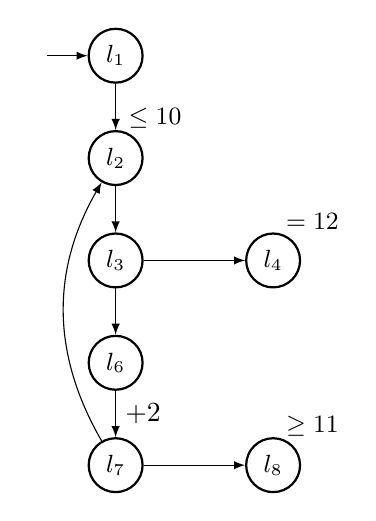
\begin{tikzpicture}[auto, >=latex, node distance = 1 cm]
				\tikzstyle{round} = [thick, draw=black, circle, font=\small]
				\tikzstyle{invis} = [draw=none, font=\small]
				
				\node[invis]			at (-1,0)		(q6)	{$ $};
				\node[round] 			at (0, 0) 		(q0) 	{$l_1$};
				\node[round] 			at (0, -1.3)	(q1) 	{$l_2$};
				\node[invis]			at (0.5, -0.8)	(c0)	{$\leq 10$};
				\node[round] 			at (0, -2.6)	(q2) 	{$l_3$};
				\node[round] 			at (2, -2.6) 	(q3) 	{$l_4$};
				\node[invis]			at (2.5, -2.1)	(c0)	{$= 12$};
				\node[round] 			at (0, -5.2)	(q4) 	{$l_7$};
				\node[round] 			at (0, -3.9)	(q7) 	{$l_6$};
				\node[round] 			at (2, -5.2)	(q5) 	{$l_8$};
				\node[invis]			at (2.5, -4.7)	(c1)	{$\geq 11$};
				
				\path[->]
				(q6)	edge				node {$ $}	(q0)
				(q0)	edge				node {$ $}	(q1)
				(q1)	edge				node {$ $}	(q2)
				(q2)	edge				node {$ $}	(q7)
				(q7)	edge				node {$+2$}	(q4)
				(q2)	edge				node {$ $}	(q3)
				(q4)	edge				node {$ $}	(q5)
				(q4)	edge [bend left]	node {$ $}  (q1);
			\end{tikzpicture}
		\end{figure}
	\end{minipage}
\end{frame}

\begin{frame}{Shortcomings}
	\begin{itemize}
		\item Does not work with variables
		\pause
		\item Can result in false positives
	\end{itemize}
\end{frame}

\section{SAT problem}

\begin{frame}{SAT problem I}
	\begin{itemize}
		\item Convert to a satisfiability problem
		\pause
		\item Can handle variables
		\pause
		\item Try to guess rather than compute
	\end{itemize}
\end{frame}

\begin{frame}{SAT problem II}
\begin{itemize}
	\item conditions
	\pause
	\begin{itemize}
		\item The initial interval needs to be $[0, 0]$
		\pause
		\item The successor function needs to be applicable to all intervals
		\pause
		\item Loops will be self satisfying 
		\pause
		\begin{itemize}
			\item One predecessor not part of loop
		\end{itemize}
	\end{itemize}
\end{itemize}
\end{frame}

\begin{frame}[fragile]{SAT problem III}
\begin{minipage}[c]{0.64\textwidth}
	\only<1>{
		\begin{table}[h]
			\footnotesize
			\begin{tabular}{ |c|c|c| }
				\hline
				p		& q 	& configuration 		\\
				\hline
				$l_1$	& $l_2$ &  	[0, 0]	\\
				\hline
				$l_2$	& $l_3$ &  	$\emptyset$\\
				\hline
				$l_3$	& $l_4$ &  	$\emptyset$\\
				\hline
				$l_3$	& $l_6$ &  	$\emptyset$\\
				\hline
				$l_6$	& $l_7$ &  	$\emptyset$\\
				\hline
				$l_7$	& $l_2$ &  	$\emptyset$\\
				\hline
				$l_7$	& $l_8$ & 	$\emptyset$\\
				\hline
			\end{tabular}
			\centering
		\end{table}
	}
	\only<2>{
		\begin{table}[h]
			\footnotesize
			\begin{tabular}{ |c|c|c| }
				\hline
				p		& q 	& configuration 		\\
				\hline
				$l_1$	& $l_2$ &  	[0, 0]	\\
				\hline
				$l_2$	& $l_3$ &  	\textcolor{red}{[0, 0]}\\
				\hline
				$l_3$	& $l_4$ &  	$\emptyset$\\
				\hline
				$l_3$	& $l_6$ &  	\textcolor{red}{[0, 0]}\\
				\hline
				$l_6$	& $l_7$ &  	\textcolor{red}{(0, 2]}\\
				\hline
				$l_7$	& $l_2$ &  	\textcolor{red}{(0, 2]}\\
				\hline
				$l_7$	& $l_8$ & 	$\emptyset$\\
				\hline
			\end{tabular}
			\centering
		\end{table}
	}
	\only<3>{
	\begin{table}[h]
		\footnotesize
		\begin{tabular}{ |c|c|c| }
			\hline
			p		& q 	& configuration 		\\
			\hline
			$l_1$	& $l_2$ &  	[0, 0]	\\
			\hline
			$l_2$	& $l_3$ &  	\textcolor{red}{(1, 10]}\\
			\hline
			$l_3$	& $l_4$ &  	$\emptyset$\\
			\hline
			$l_3$	& $l_6$ &  	\textcolor{red}{(1, 10]}\\
			\hline
			$l_6$	& $l_7$ &  	\textcolor{red}{(1, 12]}\\
			\hline
			$l_7$	& $l_2$ &  	\textcolor{red}{(1, 12]}\\
			\hline
			$l_7$	& $l_8$ & 	[11, 12]\\
			\hline
		\end{tabular}
		\centering
	\end{table}
	}
	\only<4>{
	\begin{table}[h]
		\footnotesize
		\begin{tabular}{ |c|c|c| }
			\hline
			p		& q 	& configuration 		\\
			\hline
			$l_1$	& $l_2$ &  	[0, 0]	\\
			\hline
			$l_2$	& $l_3$ &  	\textcolor{ForestGreen}{(0, 10]}\\
			\hline
			$l_3$	& $l_4$ &  	$\emptyset$\\
			\hline
			$l_3$	& $l_6$ &  	\textcolor{ForestGreen}{(0, 10]}\\
			\hline
			$l_6$	& $l_7$ &  	\textcolor{ForestGreen}{(0, 12]}\\
			\hline
			$l_7$	& $l_2$ &  	\textcolor{ForestGreen}{(0, 12]}\\
			\hline
			$l_7$	& $l_8$ & 	[11, 12]\\
			\hline
		\end{tabular}
		\centering
	\end{table}
	}
\end{minipage}
\hfill
\begin{minipage}[c]{0.35\textwidth}
	\begin{figure}[h!]
		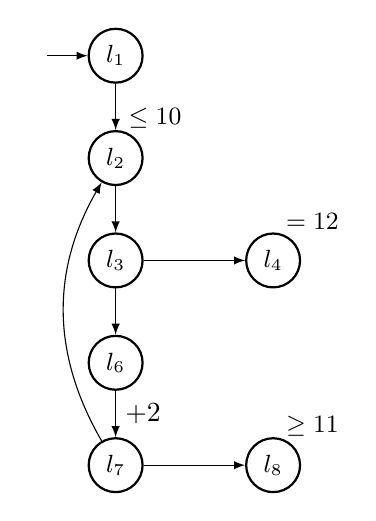
\begin{tikzpicture}[auto, >=latex, node distance = 1 cm]
			\tikzstyle{round} = [thick, draw=black, circle, font=\small]
			\tikzstyle{invis} = [draw=none, font=\small]
			
			\node[invis]			at (-1,0)		(q6)	{$ $};
			\node[round] 			at (0, 0) 		(q0) 	{$l_1$};
			\node[round] 			at (0, -1.3)	(q1) 	{$l_2$};
			\node[invis]			at (0.5, -0.8)	(c0)	{$\leq 10$};
			\node[round] 			at (0, -2.6)	(q2) 	{$l_3$};
			\node[round] 			at (2, -2.6) 	(q3) 	{$l_4$};
			\node[invis]			at (2.5, -2.1)	(c0)	{$= 12$};
			\node[round] 			at (0, -5.2)	(q4) 	{$l_7$};
			\node[round] 			at (0, -3.9)	(q7) 	{$l_6$};
			\node[round] 			at (2, -5.2)	(q5) 	{$l_8$};
			\node[invis]			at (2.5, -4.7)	(c1)	{$\geq 11$};
			
			\path[->]
			(q6)	edge				node {$ $}	(q0)
			(q0)	edge				node {$ $}	(q1)
			(q1)	edge				node {$ $}	(q2)
			(q2)	edge				node {$ $}	(q7)
			(q7)	edge				node {$+2$}	(q4)
			(q2)	edge				node {$ $}	(q3)
			(q4)	edge				node {$ $}	(q5)
			(q4)	edge [bend left]	node {$ $}  (q1);
		\end{tikzpicture}
	\end{figure}
\end{minipage}
\end{frame}

\begin{frame}{SAT problem IV}
\begin{itemize}
	\item Requires a large amount of variables
	\pause
	\begin{itemize}
		\item Four variables per interval
		\pause
		\item Two variables per node condition
		\pause
		\item Three variables per edge
	\end{itemize}
	\pause
	\item Slower than the first approach
	\pause
	\item Can give false positives
	\pause
	\item Only use SAT in case parameters are present
\end{itemize}
\end{frame}

\section{Use case: Xrdp}

\begin{frame}{Use case: Xrdp}
	\begin{itemize}
		\item Graphical login to remote machines using RDP
		\pause
		\item Medium-sized C project
		\begin{itemize}
			\item 94 458 lines of code
			\item 1 328 functions
		\end{itemize}
		\pause
		\item Analysed 73.42\% of the functions
		\pause
		\item 33 Convertible functions
		\pause
		\item 2 Parametric automata
	\end{itemize}
\end{frame}

\section{Manual verification}

\begin{frame}{Manual verification}
\begin{itemize}
	\item Introduce dead code in xrdp
	\pause
	\item 7 different types of dead code 
	\pause
	\item Test suite with 115 tests
\end{itemize}
\end{frame}

\section{Conclusion}

\begin{frame}{Conclusion}
	\begin{itemize}
		\item The proposed approach is capable of identifying dead code
		\pause
		\item No false negatives
		\pause
		\item Need for a different compiler
		\pause
		\item Further optimizations to the code constraints should be considered
	\end{itemize}
\end{frame}

\end{document}
